%% Master Thesis Template
%% Please update the specification through this link: https://daim.idi.ntnu.no/howto_thesis_submission.pdf

\documentclass[pdftex,10pt,b5paper,twoside]{book}
\usepackage[lmargin=25mm,rmargin=25mm,tmargin=27mm,bmargin=30mm]{geometry}

\usepackage{setspace}
\usepackage{graphicx}
\usepackage{amssymb}
\usepackage{mathrsfs}
\usepackage{amsthm}
\usepackage{amsmath}
\usepackage{color}
\usepackage[Rejne]{fncychap}
\usepackage[pdftex,bookmarks=true]{hyperref}
\usepackage[pdftex]{hyperref}
\hypersetup{
    colorlinks,%
    citecolor=black,%
    filecolor=black,%
    linkcolor=black,%
    urlcolor=black
}
\usepackage[font=small,labelfont=bf]{caption}
\usepackage{fancyhdr}
\usepackage{times}
\usepackage{float}
\restylefloat{figure}

% Setup references
\usepackage[backend=bibtex]{biblatex}
\addbibresource{bibfiles/bibtexlibs.bib}

\newcommand{\HRule}{\rule{\linewidth}{0.5mm}}

\renewcommand*\contentsname{Table of Contents}

\pagestyle{fancy}
\fancyhf{}
\renewcommand{\chaptermark}[1]{\markboth{\chaptername\ \thechapter.\ #1}{}}
\renewcommand{\sectionmark}[1]{\markright{\thesection\ #1}}
\renewcommand{\headrulewidth}{0.1ex}
\renewcommand{\footrulewidth}{0.1ex}
\fancypagestyle{plain}{\fancyhf{}\fancyfoot[LE,RO]{\thepage}\renewcommand{\headrulewidth}{0ex}}

\usepackage[caption=false,font=footnotesize]{subfig}

% My custom directives
%\usepackage{todonotes}

\newcommand{\cm}[1]{
    CITATION MISSING: #1
    %\todo[inline, color=cyan]{Citation missing: #1}
}

\newcommand{\todo}[1]{
    TODO: #1
}

\usepackage{tikz}

\usetikzlibrary{external}
\tikzexternalize[prefix=precompiled-figures/]

\usetikzlibrary{shapes, arrows, fit, calc}
\tikzset{vertex/.style = {shape=circle,draw,minimum size=2em}}
\tikzset{edge/.style = {->, > = latex'}}
\tikzset{box/.style = {shape=rectangle,draw, minimum size=1.5cm}}

\usepackage{pgfplots}
\pgfplotsset{compat=newest}
\usepgfplotslibrary{statistics}

% #1=\addplots #2=scalefactor for ticks #3=Label
\newcommand{\myboxplot}[4]{
  \begin{tikzpicture}
    \pgfplotsset{
      boxplot/every box/.style={fill=gray},
      boxplot/every whisker/.style={fill=black, color=black},
      boxplot/box extend=0.7
    }
    \begin{axis}
      [
        axis x line=bottom,
        axis y line=left,
        xmin=-1,
        xmax=#4,
        ymin=0.4,
        ymax=1.05,
        ytick={0.4, 0.5, 0.6, 0.7, 0.8, 0.9, 1.0},
        scaled x ticks={real:#2},
        axis y discontinuity=crunch,
        xtick scale label code/.code={},
        boxplot/draw direction=y,
        xlabel=#3,
        ylabel=Accuarcy
      ]
      #1
    \end{axis}
  \end{tikzpicture}
}


% #1=table data #2=xlabel
\newcommand{\myscatterplot}[2]{
    \begin{tikzpicture}
        \begin{axis}
            [
                axis x line=bottom,
                axis y line=left,
                axis y discontinuity=crunch,
                ymin=0.3, ymax=1.1,
                ytick={0.3, 0.4, 0.5, 0.6, 0.7, 0.8, 0.9, 1.0},
                ylabel=Accuracy,
                xlabel=#2
            ]
            \addplot[scatter src=explicit, only marks, mark size=0.5pt]
            table {#1};
        \end{axis}
    \end{tikzpicture}
}

% #1=data #2=xlabel #3=ylabel
\newcommand{\myheatmap}[3]{
    \begin{tikzpicture}
        \begin{axis}
            [
                xlabel=#2,
                ylabel=#3,
                ymax=25,
                xmax=15,
                colormap/jet,
                colorbar,
                view={0}{90}
            ]
            \addplot3[surf, shader=flat]
            file {#1};
        \end{axis}
    \end{tikzpicture}
}


\begin{document}

\frontmatter

%% PART 1
%%The title page will be automatically generated and added by the DAIM system

%% PART 2
\section*{\Huge Abstract}
\addcontentsline{toc}{chapter}{Abstract}
$\\[0.5cm]$
%Working title: "RBN as A Model for Matter Reservoirs".

% Introduction
\noindent Reservoir Computing, a relatively new approach to machine learning,
utilizes untrained recurrent neural nets as a reservoir of dynamics to preprocess some temporal task,
making it separable with a linear readout layer
Originating from the study of Liquid State Machines and Echo State Networks,
potentially any sparsely connected network containing feedforward and feedback loops can be a reservoir.
Random Boolean Networks are such sparsely connected network that may be suitable for Reservoir Computing.

% Problemstilling
Reservoir Computing can be used with physical or simulated reservoirs.
When using nontraditional physical devices for computation,
as in evolution-in-materio,
one is often restricted in how one can perturb and read out the underlying substrate.
Random Boolean network reservoir computing systems (RRC systems) may be a useful abstraction over a physical device.

% Method
The properties of these RRC systems are investigated with a series of experiments simulated in a self developed reservoir computing toolbox.
The findings are discussed in light of physical reservoirs,
with the end goal of using RBNs as a model for matter reservoirs.

% Resultater
Experiments confirm that the required reservoir size increases with the difficulty of the task at hand,
with the largest factor being how many bits of input the reservoir is required to remember.
Simulation of RRC systems can therefore aid in deciding the optimal size of physical reservoirs,
given a bridge between the computational power of the reservoir and RBNs can be deduced.

Optimal reservoir perturbance is found to lie at roughly 50\% of the size of the reservoir for RBNs with $K=3$.
When using smaller slices of a reservoir for computation,
lower amounts of total perturbation will be required as long as these perturbations are located within the same topological area.

Results also show that subsets of larger reservoirs will perform at least as well as a separate reservoir of equal size.
Any interference from the unused parts of the reservoir is either minimal or slightly positive.

Finally, no relationship is found between the attractors of an RBN and its performance in a RRC system.
It can therefore not be used for guiding the construction of accurate RBNs.

\cleardoublepage

\section*{\Huge Sammendrag}
\addcontentsline{toc}{chapter}{Sammendrag}
$\\[0.5cm]$

\noindent Write your summary here...

\cleardoublepage


\section*{\Huge Acknowledgements}
\addcontentsline{toc}{chapter}{Acknowledgements}
$\\[0.5cm]$

I would like to thank my advisor Professor Gunnar Tufte for sharing his knowledge with me,
and guiding my research through this weird and awesome part of Computer Science.

I would like to thank Porter Robinson for the album Worlds which provided the soundtrack for my final week of writing.

\clearpage


\input{listings.tex}
%\input{abbreviations.tex}	%% Optional

% Trenger ikke forklare hva alt er, men introduser begrepene
% Må ha evo-mamterio hva er introduksjon? Hvor mye stuff, mikroelektrodearray.
% Complex systems properties osv.
% Limited access to perturbation, ilmited access to information. Snapshot quantum mamterials.

\mainmatter
\chapter{Introduction}

Reservoir Computing (RC) is a category of machine learning that sprang out from the study of recurrent neural networks (RNNs).
In short, it utilizes the dynamics of some complex system dubbed a 'reservoir' to preprocess a timeseries problem,
transforming it from a temporal to a spacial one in the reservoir,
making it separable with a simple readout layer \cite{lukovsevivcius2012reservoir}.

Reservoir Computing can be used both with physical and theoretical reservoirs.
The original theoretical Echo State Networks \cite{jaeger2002adaptive} and Liquid State Machines \cite{natschlager2002liquid} provided the original basis for theoretical Reservoir Computing systems.
As alternative abstractions to RRNs,
both Cellular Automata \cite{yilmaz2014reservoir} and Random Boolean Networks \cite{rbn-reservoir} were introduced and sucessfully used in reservoir computing frameworks.
RBNs \cite{gershenson2004introduction} are an useful abstraction over many physical phenomena,
most famously used by Kauffman \cite{kauffman1969metabolic} as a model for the genetic regulatory network.
In the authors pre-thesis paper,
findings from \cite{rbn-reservoir} were reproduced and the reusability of trained readout layers investigated.
A a neturality in the state-space of possible RBNs was discovered.

Physical reservoirs take many shapes and forms.
In the ever-so-cited 'Pattern recognition in a bucket' paper \cite{fernando2003pattern},
the authors use a bucket of water to successfully perform speech recognition.
In \cite{farstad2015evolving},
a carbon-nanotube based substrate is successfully used to evolve binary logic gates as well as stable Cellular Automata.
These can then be used to build a CA-based computing paradigm over this unconventional hardware.
As Cellular Automata are a special case of Random Boolean Networks,
any general findings about RBN RC systems may be applicable to RC systems using CAs.
The wider category of attempting to harness the power of unconventional physical devices for computation,
usually aided by artificial evolution,
is known as evolution-in-materio \cite{miller2002evolution}.

When using nontraditional physical devices for computation, as in evolution-in-materio,
one is often restricted in how one can perturb and read out the underlying substrate.
It might be prohibitively expensive or technologically infeasible to read the entire state of the reservoir,
and the values sampled might be affected by its neighborhood in unknown ways to us.
In \cite{demarse2005adaptive} the authors use living rat neurons in a microelectrode array to control an airplane in a flight simulator.
Only subsets of the computational substrate are used,
and the neuronal connections even change over time.
In addition, the microelectrode array presents a limited resolution view of the computational substrate.
Questions include how the unused parts of the reservoir impact the parts used for computation,
and how large the reservoir actually needs to be to solve the task at hand.

It has been shown that Reservoir Computing using Random Boolean Networks is a feasible approach to solving binary time-series problems,
as well as being a potentially useful abstraction over physical Reservoir Computing devices.
In this thesis, the properties of these RRC systems are further investigated,
with the motivation of using the results as a template for instrumenting and performing computations on physical Reservoir Computing systems.

The following questions will be answered in this thesis:
\begin{enumerate}
    \item How small can a RRC system be while still solving its task at $ \geq 98\% $ accuracy?
    \item Does the optimal amount of reservoir perturbation depend on the task at hand?
    \item Does one have to read the state of the entire reservoir to maintain task accuracy?
    \item Is there a correlation between the topological characteristics of the RBN (number of attractors, attractor length) and its performance as a reservoir?
\end{enumerate}

Questions two and three are of specific interest to the implementation of physical reservoirs and evolution-in-materio devices.
What these approaches have in common is that physical substrates,
with varying degrees of perturbation ability and insight into the internal state,
are used for computation.
Their couplings to theoretical frameworks such as Reservoir Computing motivate the exploration of the effects of limited perturbation and readout possibilities on reservoir performance.

\section{Thesis structure}

The thesis is structured as follows:
Chapter \ref{chapter:background} provides background information on reservoir computing, random boolean networks, evo-materio, and using RBNs for Reservoir Computing.
Chapter \ref{chapter:methodology} describes the experimental setup and methodology used for performing experiments.
Chapter \ref{chapter:experiments} contains an in-depth descriptions of each experiment,
the results obtained, and a discussion thereof.
Chapter \ref{chapter:conclusion} concludes the thesis and mentions further work.


\chapter{Background}
\label{chapter:background}

\section{A Brief Introduction to Reservoir Computing}
\label{section:reservoir-computing-introduction}

Recurrent Neural Networks (RNNs), as opposed to feed-forward neural networks,
are notoriously time consuming and difficult to train \cite{Schrauwen2007}.
This is due to feedback from the recurrent connections during the training process,
allowing small topology changes to drastically change a network's position in the fitness landscape.

It was therefore proposed in both \cite{jaeger2002adaptive} (as Echo State Networks, or ESN)
and \cite{natschlager2002liquid} (as Liquid State Machines, or LSM) to separate the RNN into two parts,
the untrained reccurrent reservoir, and the trained readout layer.
Both of these methods have been unified into the field of Reservoir Computing,
now focusing on the separate training and evolution of the recurrent and readout parts \cite{lukovsevivcius2012reservoir}.
Exiting applications of Reservoir Computing include speech and handwriting recognition,
as well as controlling robotics \cite{lukovsevivcius2012reservoir}.

\begin{figure}[ht]
    \caption{
        Schematic of a general Reservoir Computing system containing adjustable biases, feedback loops, reservoir and readout layers,
        which are described in section \ref{section:reservoir-computing-introduction}.
        Inspired by figures from \cite{Schrauwen2007} and \cite{Jaeger:2007}.
    }
    \label{fig:rc-schema}
    \includegraphics[width=\columnwidth]{background/reservoir_computing_schema.pdf}
\end{figure}

A generalized structure of a Reservoir Computing system with all bells and whistles is shown in figure \ref{fig:rc-schema}.
The main components are the reservoir and the readout layer.
At each timestep in the core model,
the reservoir receives the current input signal as well as its previous state (it is recurrent after all).
It transforms it, and passes it on to the readout layer.
The output layer frequently receives the teacher input as well.
The internal weights of the reservoir are usually randomized and left untrained,
with the weights of the readout layer being adjusted by some learning algorithm.
This can be linear or ridge regression for offline learning,
or recursive least sqares for online learning \cite{Schrauwen2007}.

There are many extensions to the base model.
The reservoir and output layers can receive biases:
The readout bias is used for regularizing the reservoir state in case the problem is ill-posed,
but isn't needed when using a model like ridge regression, which performs regularization internally \cite{Schrauwen2007}.
Reservoir bias is used for stabilizing models which feeds the output layer back into the reservoir,
which may be needed if the problem entails producing oscillating output \cite{Jaeger:2007}.
Teacher forcing,
that is forcing the states of the output layer to those expected by the trainer for the first n timesteps,
usually speed up the convergence of the learning method used,
and may in some cases be required to at all achieve stability \cite{jaeger2002tutorial}.

For a deeper dive into Reservoir Computing,
consult papers \cite{Schrauwen2007}, \cite{lukovsevivcius2012reservoir}, and \cite{Jaeger:2007}.

\section{Alternatives to Classical Reservoirs}

Are there other types of complex systems that can be used as reservoirs?
What properties must these reservoirs have to be able to solve problems?

Complex networks similar to the sparsely connected RNNs used  ESN and LSM systems include Cellular Automata \cite{wolfram2002new} and Random Boolean Networks \cite{kauffman1969metabolic}.
Cellular Automata are regular grids of cells containing some state,
each cell connected to its neighbors in the grid.
Cells then update in lockstep according to some shared transition table,
creating a new generation.
RBNs can be seen upon as an abstraction over CAs again,
allowing for nonlocal neighbors and variable updating rules.
They will be introduced in depth in section \ref{section:rbns}.

Both CAs and RBNs have successfully been used in Reservoir Computing systems \cite{yilmaz2014reservoir} \cite{rbn-reservoir}.
Both models are simple, and can be implemented in software,
hardware (FPGAs), and in materio \cite{miller2002evolution} \cite{farstad2015evolving}.

This computational paradigm is known as Cellular Computing,
and provides a potentially powerful alternative to classical computers,
leveraging extreme parallelism, simple components and local state \cite{sipper1999emergence}.

\section{A Brief Introduction to Boolean Networks}
\label{section:rbns}

Random Boolean Networks, also known as Kaffman networks,
were originally developed as a model of gene regulatory networks \cite{kauffman1969metabolic},
the complex system that regulates how genes in multicellular organisms interact with each other.
The model requires no assumptions about the inner workings of the actual nodes,
which allows it to model phenomena where the exact internal workings of the system may be unknown.

The simplification of a system to a boolean model doesn't pose a problem,
as any multi-valued network can be transformed to a corresponding binary one.

A RBN is usually described by its number of nodes $N$ and the in-degree $K$ of the nodes,
that is, how many nodes each node depends on (also known as its ancestors).
RBNs can have both homogenous and heterogenous in-degrees.
In heterogenous networks, one usually describes the average connectivity $\langle K \rangle$ instead.

Each node can have a state of zero or one.
The next state of the node is solely determined by the current combination of states of its ancestors.
Each combination leads to a new state of zero or one,
with the probability given by a binomial distribution usually having $\langle P \rangle = 0.5$.
Figure \ref{figure:sample-homogenous-rbn} visualizes a homogenous RBN with $N=3, K=2, P=0.5$.

\begin{figure}
  \centering
  \subfloat[RBN topology]{
    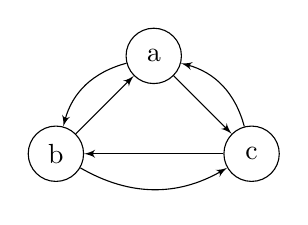
\begin{tikzpicture}[node distance = 5em]
      \node[vertex] (a) {a};
      \node[vertex] (b) [below left of=a] {b};
      \node[vertex] (c) [below right of=a] {c};

      \draw[edge] (a) to[bend right] (b);
      \draw[edge] (a) to (c);

      \draw[edge] (b) to (a);
      \draw[edge] (b) to[bend right] (c);

      \draw[edge] (c) to[bend right] (a);
      \draw[edge] (c) to (b);
    \end{tikzpicture}
  }
  \subfloat[Transition table for node a]{
    \begin{tabular}[b]{ c c | c}
      \multicolumn{2}{c}{Ancestor states} & New state \\
      \hline
      0 & 0 & 0 \\
      0 & 1 & 1 \\
      1 & 0 & 0 \\
      1 & 1 & 1 \\
    \end{tabular}
  }
  \caption{An example homogenous RBN with $N=3, K=2, P=0.5$.}
  \label{figure:sample-homogenous-rbn}
\end{figure}

In the simplest RBN updating scheme, all nodes update in lockstep.
This is known as the Classical RBN updating scheme (CRBN).
The states of the RBN at the next timestep $t+1$ therefore only depend on the states at the previous timestep $t$.
As the number of RBN states is finite ($2^{n\_nodes}$),
the system will eventually revisit a previously visited state.
This set of repeating states is known as an \emph{attractor},
and a deterministic system cannot escape from it.
If the attractor consists of a single state it is known as a point attractor,
otherwise a cycle attractor.
The set of states leading towards an attractor is known as its \emph{basin of attraction}.
A cycle attractor can be observed in figure \ref{figure:rbn-critical},
while a point attractor is observed in figure \ref{figure:rbn-ordered}.

A criticism of the classical model is that gene regulation networks are updating continiously,
as opposed to in lockstep \cite{gershenson2004introduction}.
There are therefore a number of alternate updating schemes which can be categorized by whether they are deterministic or nondeterministic, as well as synchronous and asynchronous.

The dynamics of an RBN can be categorized as being in either the ordered, critical, or chaotic phase.
These phases can be identified by how large a part of the network state is able to change over time,
whether similar states tend to converge or diverge over time,
and the networks resistance to perturbations (outside changes to the network).

One way to obtain these phases analytically is by comparing the resulting states of two identical RBNs where one is subject to some perturbation \cite{gershenson2004introduction}.
For visual identification, we plot the states of the RBN in a square lattice,
with the network states plotted horizontally, and time flowing downwards.
A node is drawn as white if its state is one, black otherwise.
The phases are visualized in Figure \ref{figure:rbn-phases}.

\begin{figure}
  \subfloat[Ordered phase, K=1]{
    \includegraphics[width=0.3\columnwidth]{background/ordered-phase.pdf}
    \label{figure:rbn-ordered}
  }
  \subfloat[Critical phase, K=2]{
    \includegraphics[width=0.3\columnwidth]{background/critical-phase.pdf}
    \label{figure:rbn-critical}
  }
  \subfloat[Chaotic phase, K=3]{
    \includegraphics[width=0.3\columnwidth]{background/chaotic-phase.pdf}
    \label{figure:rbn-chaotic}
  }

  \caption{
    Trajectories through state-space for RBNs with $N=30, K=[1,2,3]$, visualizing the different phases.
    Time flows downwards the lattice, while RBN states are shown along the X-axis.
    with the network states plotted horizontally, and time flowing downwards.
    Images created with the developed RBN-simulator.
  }
  \label{figure:rbn-phases}
\end{figure}

In general, RBNs in the critical phase are the most interesting.
These are seemingly able to support information transmission, storage and modification,
all capacities required for computation \cite{langton3computation}.
Critical systems are found on the edge of chaos,
on the phase transition between ordered and chaotic networks \cite{gershenson2004introduction}.
For RBNs with $\langle p \rangle = 0.5$,
critical dynamics are usually found at $\langle K \rangle = 2$ \cite{gershenson2004introduction},
although one could still find networks with such dynamics for different values of $\langle K \rangle$.

A thorough introduction to the field of RBNs is available in \cite{gershenson2004introduction}.

\section{RBN Reservoir systems}
\label{subsection:rbn-reservoir-systems}

How does one adapt a RBN for use as a reservoir in a RBN-RC device?
RBNs aren't usually designed to take external input.
We do however, have the concept of perturbation,
the external flipping of bits in the network's state,
transition tables or edges.
This can be utilized to create RBNs that take input,
by continiously perturbing the RBN nodes by the bits of the input sequence.

Questions that follow are how many bits should the network consume at a time,
how many of the network nodes should be perturbed by the input at each timestep,
and what dynamics must such a reservoir have to allow for the computation of interesting problems?

\subsection{A working system}

In \cite{rbn-reservoir} the authors create and analyze functioning RBN-RC systems.
\todo{Shortly mention my pre-thesis project here perhaps?}
These RBN-RC systems have heterogenous connectivity,
consume one bit of input at each timestep ($I=1$),
perturbing $IC$ of the $N$ nodes in the process.
The readout layer can be any node performing some kind of regression of the reservoir state against expected outout for the current task, e.g. linear regression.
Such a setup is shown in Figure \ref{figure:rbn-reservoir}.

\begin{figure}
  \centering
  \includegraphics[width=\columnwidth]{background/RBN-Reservoir.pdf}
  \caption{
    RBN-Reservoir system with $I=1, IC=2, K=2, N=6$ with the entire reservoir sate used for regression.
    The reservoir transforms the problem from a temporal one to a multidimentional spatial one.
    The readout layer the performs some kind of learning on the reservoir states against the expected output for the current task.}
  \label{figure:rbn-reservoir}
\end{figure}

\subsection{Tasks}
\label{section:tasks}

To measure the real-life performance and accuracy of the RBN Reservoir systems,
two tasks were introduced: Temporal Density and Temporal Parity \cite{rbn-reservoir}.
Both require the reservoir to be able to retain information for a sliding window of size $ n $,
offset by some value $ t $, back through the input stream.
The Temporal Parity task requires us to determine if there were an odd number of ones in the sliding window,
the Temporal Density task to determine whether there were a majority of ones.
The Former is visualized in figure \ref{figure:temporal-parity}.

Both tasks will be used to benchmark the reservoirs created later in this paper.

\begin{figure}
  \subfloat[Input]{
    \includegraphics[width=\columnwidth]{background/temporal_parity-10-200-3-input.pdf}
  }

  \subfloat[Correct output]{
    \includegraphics[width=\columnwidth]{background/temporal_parity-10-200-3-output.pdf}
  }

  \caption{
    The first 30 elements of a Temporal Parity task with $[n=3, t=0]$.
    A one is visualized as white, while a zero is black.
    We see that correct output at time $i$ is equal to there being an odd number of $1$s in inputs $[i, i-1, i-2]$
  }
  \label{figure:temporal-parity}
\end{figure}

\subsection{Computational capability}
\label{section:computational-capability}
For an RBN-reservoir to perform well at computational tasks,
it must be able to both forget past perturbations and keep two input streams that have begun converging separated \cite{bertschinger2004real}.

These two properties are coined \textit{fading memory} and \textit{separation property},
and can be measured \cite{rbn-reservoir} as follows.

Create two equal input streams \#1 and \#2 of length $T$.
If measuring \textit{fading memory}, flip the first bit in stream \#2.
If measuring \textit{separation property}, flip all bits up to bit $T-t$ in stream \#2
($t$ being the required depth of separation).
For both input streams, reset reservoir state, perturb the reservoir with the input stream,
and store the final state.
The score of the measure is then defined as the normalized hamming distance between the resulting states.
The computational capability $\Delta$ of an RBN-reservoir is then defined as
\begin{equation}
  \Delta_{Tt} = separation\_property_{Tt} - fading\_memory_{T}
\label{formula:accuracy}
\end{equation}
Analyzing different RBN-reservoirs with this metric \cite{rbn-reservoir},
a high $\Delta$ is found to correlate with critical connectivity ($\langle K \rangle = 2$).
For all RBN-reservoirs, $\Delta$ drops when increasing the required separation $t$,
and is maximized when one doesn't have to remember anything at all ($t=0$).

\subsection{Optimal perturbance}
\label{section:optimal-perturbance}
It is found that the optimal amount of reservoir perturbance,
adjustable by the number of connections between the input layer and the reservoir,
depends on both the task size, how many steps in time are required to be remembered,
and the dynamics of the reservoir.
\textit{Chaotic reservoirs} require few input connections to be able to properly spread information,
but perform poorly on larger tasks due to past perturbations still floating around the reservoir.
\textit{Ordered reservoirs} quickly forget past perturbations, allowing some success for larger tasks,
but their inability to remember past perturbations renders them useless for many tasks.
\textit{Critical reservoirs} require connectivity somewhere in the middle.
Able to forget as well as remember, they perform accurately independent of task size.

\section{Evo Materio, water bucket}
\todo{Gotta write about Evo Materio. I'm a bit unsure where to put this section in the background chapter,
and what angle it should have-if any- that's different from just showing some physical reservoir systems}

\section{RBN Reservoir Computing systems in the authors pre-thesis project}
\label{section:pre-thesis-project}

In his pre-thesis paper, the author investigated the dynamics, performance, and viability of RBNs used for Reservoir Computing (RRC).
A functioning RBN Reservoir Computing system was implemented,
and its results validated against and found in accordance with those from \cite{rbn-reservoir}.
This self-written framework serves as the basis for the simulations and analysis perfored in this thesis as well.

A positive correlation between the computational capability (section \ref{section:computational-capability}) of a reservoir and its actual performance is found.
The optimal connectivity for homogenous reservoirs is found to be $K=3$ as opposed to $\langle K \rangle = 2$ for heterogenous reservoirs \cite{rbn-reservoir}.
Finally, the required input connectivity is found to rise with the presence of chaotic dynamics in the reservoir.
The figures backing this conclusion are shown in \ref{figure:results:temporal-parity-3} and \ref{figure:results:temporal-parity-5}.

Finally, a one-to-many mapping between the readout layer in an already-trained RRC system and different RBN reservoirs was found,
with there being a seemingly large set of interchangeable reservoirs for each readout layer.
This makes the potential use of a smaller generative genome for evolving RRC systems interesting.
Even though it hits fewer points in the RBN fitness landscape than the fixed genome used in this paper,
a large amount of these points are still usable for each instance of a working readout layer.

\begin{table}[ht]
    \centering
    \caption{Task parameters for the pre-thesis project.}
    \label{table:pre-thesis-tasks}
    \begin{tabular}{ll}
        \hline
        \textbf{Parameter} & \textbf{Configuration} \\
        \hline
        \hline
        Task type               & Temporal Parity \\
        Training dataset length & 4 000                       \\
        Test dataset length     & 200                         \\
        $N$ (window size)       & 3 and 5                     \\
        $t$ (offset)            & 0 \\
        \hline
    \end{tabular}
\end{table}

\begin{figure*}[!t]
    \centering
    \caption{
        Plots for Temporal Parity with $N=3$ (parameters in table \ref{section:tasks}).
        Figures \ref{fig:res:d-100-3-1}--\ref{fig:res:d-100-3-3} plot the accuracies of the sampled RBNs against their input connectivity,
        for K=1–3 respectively.
        Figures \ref{fig:res:c-100-3-1}--\ref{fig:res:c-100-3-3} plot the accuracy of the previous figures against their Computational Capability ($T=100, t=3$).
    }
    \label{figure:results:temporal-parity-3}
    \resizebox{\textwidth}{!}{
        \subfloat[K=1]{
            \label{fig:res:d-100-3-1}
            \input{background/pre-project/distribution-100-3-1.tex}
        }
        \subfloat[K=1]{
            \label{fig:res:c-100-3-1}
            \myscatterplot{background/pre-project/computational-power-100-3-1.dat}
        }
    }

    \resizebox{\textwidth}{!}{
        \subfloat[K=2]{
            \label{fig:res:d-100-3-2}
            \input{background/pre-project/distribution-100-3-2.tex}
        }
        \subfloat[K=2]{
            \label{fig:res:c-100-3-2}
            \myscatterplot{background/pre-project/computational-power-100-3-2.dat}
        }
    }

    \resizebox{\textwidth}{!}{
        \subfloat[K=3]{
            \label{fig:res:d-100-3-3}
            \input{background/pre-project/distribution-100-3-3.tex}
        }
        \subfloat[K=3]{
            \label{fig:res:c-100-3-3}
            \myscatterplot{background/pre-project/computational-power-100-3-3.dat}
        }
    }
\end{figure*}

\begin{figure*}[!t]
    \centering
    \caption{
        Plots for Temporal Parity with $N=5$ (parameters in table \ref{section:tasks}).
        Figures \ref{fig:res:d-100-5-1}--\ref{fig:res:d-100-5-3} plot the accuracies of the sampled RBNs against their input connectivity,
        for K=1–3 respectively.
        Figures \ref{fig:res:c-100-5-1}--\ref{fig:res:c-100-5-3} plot the accuracy of the previous figures against their Computational Capability ($T=100, t=3$).
    }
    \label{figure:results:temporal-parity-5}
    \resizebox{\textwidth}{!}{
        \subfloat[K=1]{
            \label{fig:res:d-100-5-1}
            \input{background/pre-project/distribution-100-5-1.tex}
        }
        \subfloat[K=1]{
            \label{fig:res:c-100-5-1}
            \myscatterplot{background/pre-project/computational-power-100-5-1.dat}
        }
    }

    \resizebox{\textwidth}{!}{
        \subfloat[K=2]{
            \label{fig:res:d-100-5-2}
            \input{background/pre-project/distribution-100-5-2.tex}
        }
        \subfloat[K=2]{
            \label{fig:res:c-100-5-2}
            \myscatterplot{background/pre-project/computational-power-100-5-2.dat}
        }
    }

    \resizebox{\textwidth}{!}{
        \subfloat[K=3]{
            \label{fig:res:d-100-5-3}
            \input{background/pre-project/distribution-100-5-3.tex}
        }
        \subfloat[K=3]{
            \label{fig:res:c-100-5-3}
            \myscatterplot{background/pre-project/computational-power-100-5-3.dat}
        }
    }
\end{figure*}

\cleardoublepage


% Background chapter - dynamical systems / reservoir computing / evo materio / boolean networks
% Background: Trenger evo materio kapittel
% Bør nevne noen som bruker fysisk reservoir som reservoir, få lenket sammen de to greierne
% Må ha seksjon som beskriver reservoir computing med boolske nettverk. Fra meg!

% Method chapter, som i forprosjekt. Motivasjon! Motivasjon!!
% Elektroder i materialet,, hvor mange, gror det, begrenset innsikt i systemet.
% Simuler dette / regne dette med å droppe output.

\chapter{Methodology}

We have shown that reservoir computing using Random Boolean Networks is a feasible approach to solving binary time-series problems.
We now wish to investigate which parameters and characteristics of the reservoir lead to optimal performance and resource usage.

The following questions arise:

\begin{enumerate}
    \item How small can a RBN Reservoir System be while still solving a given task at close to 100\% accuracy?
    \item How many connections from the input layer are required to sufficiently perturb the reservoir?
    \item How few reservoir nodes can be connected to the readout layer while maintaining task accuracy?
    \item Is there a correlation between the dynamical characteristics of the RBN (number of attractors, attractor length) and its performance as a reservoir?
\end{enumerate}

The answers to these questions aren't 'just' of theoretical interest,
they also give us insight to how physical reservoir computing devices have to be instrumented.

In a physical substrate it might be prohibitively expensive or technologically infeasible to read the state of the entire reservoir,
and the nodes you are able to measure might be affected by the 'values' of the nodes next to it.
In the case of a growing and modifying reservoir, such as a stem-cell based reservoir,
the topology of the network might change over time without having the ability to reinstrument the device.
A finding that it's enough to use a subset of the available nodes for regression in the readout layer,
regardless of reservoir size, would be of practical interest.

There are two factors affecting optimal reservoir perturbance:
There might be a problem-specific optimal perturbance dependent on the task at hand as well as connectivity of the reservoir and number of runs after each perturbance.
For physical devices one is in addition limited by the physical characteristics of the reservoir,
such as cost and the number of available electrodes for instrumenting limited by physical space.

Finding the minimum required size of a RBN Reservoir for a given task allows us to create physical reservoirs with adequate computational abilities guided by the theoretical foundations described herein ("Helmax setning, Egon! Helmax!").

Finally, we attempt to explain the performance of RBN Reservoirs through their dynamical properties,
calculating the number of attractors and their length for reservoirs against their accuracy on a given task.
A correlation between these properties might be interesting, and help to explain why some reservoirs perform better than others.

\section{Experimental setup}

The final RRC system is shown as a block diagram in Figure \ref{figure:rrc-block},
and the actual network topology is equivalent to the one in Figure \ref{figure:rbn-reservoir}.

\todo{so much todo}
\todo{Explain every box line in the box diagram, probably with more stuff}

\todo{gotta add moar stuffz here, nemlig varierende input/output cocnnectivitet støtte}

\begin{figure}
  \centering
  \begin{tikzpicture}
    \node (dataset) {Dataset};
    \node[box, below=of dataset] (input) {Input layer};
    \node[box, right=of input] (reservoir) {RBN Reservoir};
    \node[box, right=of reservoir] (readout) {Readout layer};
    \node[above=of readout] (classification) {Classification};

    \node[draw,dotted,fit=(input) (reservoir) (readout), label={RRC}] {};

    \draw[edge] (dataset) to (input);
    \draw[edge] (input) to (reservoir);
    \draw[edge] (reservoir) to (readout);
    \draw[edge] (readout) to (classification);
  \end{tikzpicture}
  \caption{Block diagram of the RRC processing a dataset.}
  \label{figure:rrc-block}
\end{figure}

\subsection{testing}

To verify that RBN simulation is working,
a RBN is created randomly, initial state set to all zeros, and ran.
The results are visualized in Figure \ref{figure:rbn-noperturb}.
We see that the RBN exhibits stable dynamics, and enters into an attractor around $t=15$.
In Figure \ref{figure:rbn-perturb} we continiously perturb the RBN with the input stream from the Temporal Parity task visualized in Figure \ref{figure:temporal-parity}.
In the perturbed case, the state trajectory is continiously changed, preventing the RBN from settling into an attractor.
Interestingly enough, there seems to be a visual similarity between the two cases.
Such a pattern is sure to dissapear with a RBN in the chaotic phase.

This erratic pattern of state transitions is then fed into the readout layer,
which is then tasked with finding a linear combination of the RBN states that results in the expected output for the given task.

\begin{figure}
  \subfloat[Unperturbed]{
    \includegraphics[width=0.5\columnwidth]{method/final-1-noperturb.pdf}
    \label{figure:rbn-noperturb}
  }
  \subfloat[Perturbed]{
    \includegraphics[width=0.5\columnwidth]{method/final-1-perturb.pdf}
    \label{figure:rbn-perturb}
  }
  \caption{
    The same RBN ($N=100, K=2, P=0.5, L=50$) shown both perturbed and unperturbed.
    The boolean states of the RBN are plotted along the X-axis,
    with time flowing downwards.
  }
\end{figure}

\subsection{Training}

To train the RRC system we require large training datasets,
as well as different, smaller datasets for testing the trained system.
We will use the datasets described in section \ref{subsection:rbn-reservoir-systems}.

We then either create a new RBN (initialize it randomly),
or load a previously created RBN from disk.
For each bit of input in each dataset,
we perturb the input-connected nodes in the RBN.
After each perturbance, the RBN is ran synchronously (CRBN mode) for one timestep.
The resulting RBN states are collected,
and after the entire dataset is processed,
forwarded to the readout layer.

To find a suitable mapping from the set of reservoir states and the correct input classification,
ridge regression \cite{hoerl1970ridge} is used.
This version of least squares regression is more accurate when faced with input colinearities, as well as always being at least as accurate as ordinary least squares.  
This process is repeated for all the datasets,
and the final regression parameters are chosen as a combination of the parameters obtained for each individual dataset.
Finally we measure the normalized accuracy of the trained reservoir on the test dataset,
defined as the following:
\begin{equation}
Accuracy = 1 - \dfrac{sum(actual\_output \neq expected\_output)}{len(correct\_output)}
\label{formula:accuracy}
\end{equation}

\section{Finding the minimum required reservoir size, optimal input connectivity}

As shown in my previous paper \cite{MyPreviousPaper},
there are a plethora of RRC systems with $N=100, K=\{2, 3\}$ that solve the Temporal Parity task for a window size of both 3 and 5,
The reservoirs with $K=3$ had a higher density of success in general,
and the larger reservoirs fared better on the task with window size 5.

Presumably the same tasks can be solved with smaller reservoirs,
the question being how small they can be while retaining accurarcy.
As the optimal reservoir size and input connectivity might depend on the task at hand,
we test our reservoirs on both the Temporal Parity \ref{missing} and Temporal Density \ref{missing}
tasks with window sizes of both 3 and 5 (as specified in table \ref{tab:tasks}).

\begin{table}[ht]
  \centering
  \caption{Task parameters}
  \label{tab:tasks}
  \begin{tabular}{ll}
    Task type               & Temporal Parity and Density \\
    Training dataset length & 4 000                       \\
    Test dataset length     & 200                         \\
    $N$ (window size)       & 3 and 5                     \\
    $t$ (offset)            & 0
  \end{tabular}
\end{table}

To find the optimal reservoir size and input connectivity,
we'll randomly initialize 50 reservoirs for each combination of the reservoir parameters in table \ref{tab:ic-reservoir-parameters}.

For our experiments we'll only be looking at reservoirs with $K=3$.
As well as being more useful due to the homogenous degree of the network (to simulate $\langle K \rangle = 2 $) and
having a higher population accuracy, it reduces the number of parameter combination we have to simulate.

\begin{table}[ht]
    \centering
    \caption{Reservoir parameters for optimal input connectivity}
    \label{tab:ic-reservoir-parameters}
    \begin{tabular}{ll}
        Nodes               & [10..50], step size=5         \\
        Connectivity        & 3                             \\
        Input connectivity  & [0..n\_nodes], step size = 5  \\
		Output connectivity & n\_nodes                      \\
        Sample size         & 50
    \end{tabular}
\end{table}

After plotting the resulting accuracies on the previously mentioned tasks,
one should be able to visually identify the minimum required reservoir size for the given task,
as well as what the optimal input connectivity might be, as a function of reservoir size and task.

\section{Minimum required output connectivity}

How few connections can one have from the reservoir itself to the readout layer,
while staying accurate on the task at hand?
As the reservoir prediction is computed by regressing the states of the network nodes against the expected output bits,
reducing the number of nodes used in the regression can never give a higher accuracy than using all of the nodes.
If there is redundant information in the network, quite a few nodes could be cut off from the readout layer while maintaining the best accuracy for this specific reservoir.
This does require a sufficient amount of linear independence between the remaining nodes of the network.

As shown in the previous section, different problems require different reservoir sizes.
Past a certain reservoir size, all reservoirs have a sufficient accuracy on the given task.
One could postulate that for reservoirs larger than the 95\% accuracy breakpoint,
it suffices to read out a number of nodes equal to the breakpoint.
If this is the case, one can safely use growing reservoirs without having to change the output connections,
given that the reservoir was able to solve the given task in the first place.

The results from the previous section show a correlation between input connectivity and accuracy,
\todo{As this information isn't really obtained before i've presented the results section for the previous task, i'm not sure how to structure it. Probably method->experiment->result for each task in succession?}
with the reservoirs having a input connectivity of $n\_nodes / 2$ having the highest population accuracy.
Using this information, we can reduce our search space for minimum required output connectivity considerably.
The parameters in table \ref{tab:oc-reservoir-parameters} will be used for simulation.

\begin{table}[ht]
    \centering
    \caption{Reservoir parameters for optimal output connectivity}
    \label{tab:oc-reservoir-parameters}
    \begin{tabular}{ll}
        Nodes               & [10..100], step size=10           \\
        Connectivity        & 3                                 \\
        Input connectivity  & $ n\_nodes / 2 $                  \\
        Output connectivity & [0..n\_nodes], step size=10       \\
        Sample size         & 50
    \end{tabular}
\end{table}

\section{Analyzing reservoir dynamics}

Analysis of Random Boolean Networks often focuses on their dymanical properties.
These include whether the network is chaotic, stable or critical,
the number of attractors, attractor size, basin size, and transient times.
For a given set of RBN parameters, one can analytically obtain bounds on the statistical averages of these values.

The accuracies of reservoirs for a given set of parameters also follow some distribution.
To find out if there is a correlation between a reservoirs dynamical properties and its accuracy on a task,
the number of attractors, their length, and transient times will be calculated alongside its accuracy on the task.

To find the number of attractors in a Random Boolean Network, there are two choices:
To exhaustively search all trajectories from all initial states untill a cycle is found,
or exploring only a subset of initial states.
For larger networks, an exhaustive search may be computationally infeasible,
with the number of initial states exponential in the size of the RBN.

As shown in paper \cm{that paper},
the means of the number of attractors and their lengths when calculated from a subset of initial states is in fact representative of the actual means for reservoirs with $K=2$.
As our reservoirs have a connectivity of $K = 3$, exhaustive search will have to be conducted instead.
\cm{Fact-check this, there's also that algorithm thats much faster than exhaustive search in that paper you found that time}.
Emprical testing shows that this limits us to reservoirs of a maximum number of 16 nodes,
enough to solve the Temporal Parity task with a window size of 3, but not for 5.
In section \ref{results-of-required-size} we see that the minimum required reservoir size for that task is closer to SOMENUNMBER.
The computationally easier Temporal Density task \ref{task-description-section},
with window sizes of both 3 and 5,
will therefore be used instead.


\chapter{Experiments}

\section{Minimum required reservoir size, optimal input connectivity}

In the chapter summarizing my previous paper \ref{background:my-previous-paper},
we saw that there was a plethora of RRC systems with $N=100, K=\{2, 3\}$ that were able to solve TP3 (Temporal Parity with a window size of 3).

With TP5, $N=100, K=3$ was barely enough for a few of the generated reservoirs to reach an accuracy of over 95\%.
In both cases the reservoirs with $K=3$ performed better than their $K=\{1, 2\}$ brethren,
with $K=3$ being requried for TP5.
A homogenous connectivity of $K=3$ will therefore be chosen as the only connectivity looked at in these experiments
It more closely approximates $\langle K \rangle = 2 $, where most critical reservoirs are found,
as well as reducing the size of the parameter space we have to search.

To find the minimum required reservoir size,
we'll be creating reservoirs with the parameters presented in table \ref{tab:ic-reservoir-parameters},
for all four task combinations presented in table \ref{tab:tasks},
namely TP3, TP5, TD3 and TD5 (TP = Temporal Parity, TD = Temporal Density, number equals window size).
Presumably the TP3 task can be solved with a much smaller reservoir,
while TP5 might require a slightly larger reservoir.
As the TD task is computationally less expensive,
we can expect a smaller required reservoir size.

\begin{table}[ht]
    \centering
    \caption{Task parameters. The tasks are explained in detail in chapter \ref{section:tasks}}
    \label{tab:tasks}
    \begin{tabular}{ll}
        Task type               & Temporal Parity and Temporal Density \\
        Training dataset length & 4 000                       \\
        Test dataset length     & 200                         \\
        $N$ (window size)       & 3 and 5                     \\
        $t$ (offset)            & 0
    \end{tabular}
\end{table}

\begin{table}[ht]
    \centering
    \caption{Reservoir parameters for optimal input connectivity}
    \label{tab:ic-reservoir-parameters}
    \begin{tabular}{ll}
        Nodes               & 10 to (100, 140) for TP, 5 to (35, 65) for TD \\
        Node step size      & 10 for TP, 5 for TD \\
        Connectivity        & 3                              \\
        Input connectivity  & [0..n\_nodes], step size = 5   \\
		Output connectivity & n\_nodes                       \\
        Sample size         & 50
    \end{tabular}
\end{table}

For each reservoir size, we'll also iterate over the input connectivities,
to find which input connectivity gives the greatest population accuracy.
In my previous paper \ref{background:my-previous-paper},
the optimal input connectivity seemed to lie at roughly $ 0.5*n\_nodes $,
with the $K=3$ reservoirs having a slight skew to the right.
The Temporal Density task might have different input connectivity requirements to the Temporal Parity task.

The resulting accuracies wil be plotted as boxplots, as previously done in \ref{background:my-previous-paper}.
This should allow for visual identification of where the optimal reservoir size lies for each task,
as well as the optimal input connectivity.

\subsection{Results}

Task accuracy thresholds,
defined as the smallest reservoir size where at least two reservoirs have the required accuracy,
are presented in figure \ref{fig:accuracy-threshold-size} and table \ref{tab:accuracy-thresholds}.
The 90\% accuracy threshold is also included in table \ref{tab:accuracy-thresholds} as it appears quite a bit earlier than the 98\% threshold for tasks with a window size of 5.

\begin{figure}[ht]
    \centering
    \caption{
        Accuracy plots for the required reservoir sizes to reach the 98\% accuracy threshold for each of the four tasks:
        TP3 (Figure \ref{fig:threshold-TP3}), TP5 (Figure \ref{fig:threshold-TP5}), TD3 (Figure \ref{fig:threshold-TD3}) and TD5 (Figure \ref{fig:threshold-TD5}).
        The x-axis for all plots has been normalized to the largest reservoir size, $N=90$.
    }
    \label{fig:accuracy-threshold-size}
    \resizebox{\textwidth}{!}{
        \subfloat[TP3, N=20]{
            \input{experiments/results/normalized-threshold-plots/boxplot-input_connectivity-N20-K3-S50.tex}
            \label{fig:threshold-TP3}
        }
        \subfloat[TP5, N=90]{
            \input{experiments/results/normalized-threshold-plots/boxplot-input_connectivity-N90-K3-S50.tex}
            \label{fig:threshold-TP5}
        }
    }
    \resizebox{\textwidth}{!}{
        \subfloat[TD3, N=10]{
            \input{experiments/results/normalized-threshold-plots/boxplot-input_connectivity-N10-K3-S50.tex}
            \label{fig:threshold-TD3}
        }
        \subfloat[TD5, N=55]{
            \input{experiments/results/normalized-threshold-plots/boxplot-input_connectivity-N55-K3-S50.tex}
            \label{fig:threshold-TD5}
        }
    }
\end{figure}

\begin{table}[ht]
    \centering
    \caption{Accuracy thresholds for all four tasks.}
    \label{tab:accuracy-thresholds}
    \begin{tabular}{lllll}
                            & TP3 & TP5 & TD3 & TD5 \\
    90\% accuracy threshold & ~15 & 70  & 10  & 30  \\
    98\% accuracy threshold & 20  & 90  & 10  & 55
    \end{tabular}
\end{table}

The number of input connectivity plots resulting from the reservoir (table \ref{tab:ic-reservoir-parameters}) and task parameter (table \ref{tab:tasks}) combinations is quite large.
Therefore only reservoir sizes of $ N=[10...30, 80...100]$ from the accuracy distributions on the Temporal Parity 3 task is shown here (figure \ref{fig:TP3-IC}).
There is a slight skew to each side of $ 0.5 * n\ _nodes $ dependent on whether the task chosen is Temporal Parity or Temporal Density.
This is observable in figure \ref{fig:TP3-IC} for TP3 and appendix \ref{app:reservoir_size-input_connectivity} figures \label{fig:TP3-IC-1} through \label{fig:TD5-IC-2} for the remaining tasks.

\begin{figure*}[ht]
    \centering
    \caption{
        Plots of input connectivity against accuracy on TP3. Reservoir sizes $[40..70]$ are omitted for brevity.
        Note that the optimal input connectivity tends slightly to the right of the middle for all reservoir sizes.
        The omitted plots are presented in figures \ref{fig:TP3-IC-1} and \ref{fig:TP3-IC-2} in appendix \ref{app:reservoir_size-input_connectivity}.
        }
    \label{fig:TP3-IC}
    \resizebox{\textwidth}{!}{
        \subfloat[N=10]{
            \input{experiments/results/TP3-IO/boxplot-input_connectivity-N10-K3-S50.tex}
        }
        \subfloat[N=80]{
            \input{experiments/results/TP3-IO/boxplot-input_connectivity-N80-K3-S50.tex}
        }
    }
    \resizebox{\textwidth}{!}{
        \subfloat[N=20]{
            \input{experiments/results/TP3-IO/boxplot-input_connectivity-N20-K3-S50.tex}
        }
        \subfloat[N=90]{
            \input{experiments/results/TP3-IO/boxplot-input_connectivity-N90-K3-S50.tex}
        }
    }
    \resizebox{\textwidth}{!}{
        \subfloat[N=30]{
            \input{experiments/results/TP3-IO/boxplot-input_connectivity-N30-K3-S50.tex}
        }
        \subfloat[N=100]{
            \input{experiments/results/TP3-IO/boxplot-input_connectivity-N100-K3-S50.tex}
        }
    }
\end{figure*}

We confirm this skew by calculating the optimal input connectivity for each task as follows:
\begin{equation} \label{eq:optimal-ic}
optimal\_ic^{task} = average(max\_accuracy\_ic_{n\_nodes}^{task} / n\_nodes)
\end{equation}
where $ max\_accuracy\_ic_{n\_nodes}^{task} $ is the connectivity which gives the highest number of high-accuracy reservoirs for that task and reservoir size.
The results are presented in table \ref{tab:optimal-ic}.

\begin{table}[h]
	\centering
	\caption{Optimal input connectivities as fraction of reservoir size.}
	\label{tab:optimal-ic}
	\begin{tabular}{lllll}
						 & $T=3$  & $T=5$ \\
        Temporal Parity  & 0.528          & 0.489         \\
        Temporal Density & 0.439          & 0.443
	\end{tabular}
\end{table}

\subsection{Discussion}

\subsubsection{Required reservoir size}

In section \ref{my previous paper} Temporal Density was experimentally found to be the more difficult task, and therefore chosen for benchmarking the reservoirs.
Reservoirs with $N=100, K=3$ were found to be overkill for TP3, while being on the edge of solving TP5.
The expected relationship between the relative difficulties of the four tasks is therefore $ TD3 <= TP3 <= TD5 <= TP5 $.
Figure \label{fig:threshold-TP3} and table \ref{tab:accuracy-thresholds} confirms this suspicion.
For the same window size, Temporal Parity requires a larger reservoir.
The additional computational requirements of being able to remember five timesteps into the past requires quite a ramp up in reservoir size.

A reservoir of size 20 is large enough for TP3 (a bit lower than the 100 nodes used in my previous paper).
$ n\_nodes = 90 $ appears sufficient for TP5, slightly lower than in the previous experiments,
although the entire accuracy distribution doesn't increase significantly untill $ n\_nodes = 120 $, as shown in figure \ref{fig:TP5-IC-2}.
For TD3, a tiny reservoir of size 10 is sufficient, with a reservoir of size 5 achieving 90\% accuracy!
There is a corresponding ramp-up in required reservoir size to 55 to achieve 98\% accuracy on TD5.

Using this knowledge and the RRC system as an abstraction over a physical RC device,
one can simulate roughly the required size of a reservoir based on the pysical reservoirs estimated connectivity.
With this knowledge, one can create a physical reservoir just the right size for the computational problem at hand.

\subsubsection{Optimal input connectivity}

Temporal Density had an optimal input connectivity of roughly 0.44, while Temporal Parity lay around 0.50.
These values differ relatively little across tasks,
which is to be expected as the reservoir connectivity is the main factor in how large a reservoir perturbance is required \cm{thatpaperwiththeoreticalcomputationsforinputconnectivity},
with higher connectivities requiring larger perturbances lest the input be lost in the chaotic transitions of the reservoir.
This knowledge can be used to assist in choosing the degree of perturbance of a real-life reservoir computing system.
If one is able to measure the connectivity of the reservoir,
one can select a reasonable starting point for the amount of reservoir perturbance.


\section{Minimum required output connectivity}

How few connections can one have from the reservoir itself to the readout layer,
while staying accurate on the task at hand?
As the reservoir prediction is computed by regressing the states of the network nodes against the expected output bits,
reducing the number of nodes used in the regression can never give a higher accuracy than using all of the nodes.
If there is redundant information in the network, quite a few nodes could be cut off from the readout layer while maintaining the best accuracy for this specific reservoir.
This does require a sufficient amount of linear independence between the remaining nodes of the network.

As shown in the previous section, different problems require different reservoir sizes.
Past a certain reservoir size, all reservoirs have a sufficient accuracy on the given task.
One could postulate that for reservoirs larger than the 95\% accuracy breakpoint,
it suffices to read out a number of nodes equal to the breakpoint.
If this is the case, one can safely use growing reservoirs without having to change the output connections,
given that the reservoir was large enough to solve the given task in the first place.

As shown in section \ref{experiments:1:results}, there is a correlation between input connectivity and accuracy.
For our reservoirs with $K=3$, the optimal input connectivity was found to be $n\_nodes/2$.
Using this information, we can reduce our search space for minimum required output connectivity.
The parameters in table \ref{tab:oc-reservoir-parameters} will be used for simulation.

\begin{table}[ht]
    \centering
    \caption{Reservoir parameters for optimal output connectivity}
    \label{tab:oc-reservoir-parameters}
    \begin{tabular}{ll}
        Nodes               & 10 to (100, 140) for TP, step size=10 \\
        Connectivity        & 3                              \\
        Input connectivity  & $ n\_nodes / 2 $               \\
        Output connectivity & [0..n\_nodes], step size=10    \\
        Sample size         & 50
    \end{tabular}
\end{table}

\subsection{Results}

\begin{figure*}[ht]
    \centering
    \caption{
        O shit.
        Comparison of accuracy of all reservoirs <= 100 to a single reservoir of size 100 where one chooses to read out a subset of the data.
    }
    \label{fig:output-connectivity-TP3}
    \resizebox{\textwidth}{!}{
        \myboxplot{

% 5 of 10
\addplot[mark=*, boxplot, boxplot/draw position=1]
table[row sep=\\, y index=0] {
data
0.785 \\
0.89 \\
0.48 \\
0.495 \\
0.62 \\
0.635 \\
0.735 \\
0.82 \\
0.495 \\
0.65 \\
0.635 \\
0.635 \\
0.73 \\
0.785 \\
0.735 \\
0.815 \\
0.65 \\
0.825 \\
0.69 \\
0.65 \\
0.515 \\
0.665 \\
0.67 \\
0.495 \\
0.495 \\
0.525 \\
0.645 \\
0.72 \\
0.755 \\
0.71 \\
0.635 \\
0.65 \\
0.535 \\
0.78 \\
0.73 \\
0.755 \\
0.775 \\
0.67 \\
0.715 \\
0.495 \\
0.485 \\
0.705 \\
0.66 \\
0.615 \\
0.495 \\
0.495 \\
0.495 \\
0.495 \\
0.87 \\
0.675 \\
};

% 10 of 20
\addplot[mark=*, boxplot, boxplot/draw position=2]
table[row sep=\\, y index=0] {
data
0.92 \\
0.995 \\
0.9 \\
0.76 \\
0.945 \\
0.575 \\
0.96 \\
0.925 \\
0.96 \\
0.995 \\
0.61 \\
0.625 \\
0.615 \\
0.78 \\
0.995 \\
0.885 \\
0.785 \\
0.955 \\
0.995 \\
0.735 \\
0.87 \\
0.94 \\
0.81 \\
0.63 \\
0.995 \\
0.465 \\
0.525 \\
0.525 \\
0.97 \\
0.72 \\
0.55 \\
0.94 \\
0.965 \\
0.885 \\
0.665 \\
0.935 \\
0.7 \\
0.94 \\
0.8 \\
0.66 \\
0.815 \\
0.81 \\
0.87 \\
0.77 \\
0.895 \\
0.945 \\
0.845 \\
0.955 \\
0.925 \\
0.765 \\
};

% 15 of 30
\addplot[mark=*, boxplot, boxplot/draw position=3]
table[row sep=\\, y index=0] {
data
0.99 \\
0.755 \\
0.96 \\
0.85 \\
0.825 \\
0.995 \\
0.995 \\
0.62 \\
0.79 \\
0.77 \\
0.97 \\
0.95 \\
0.915 \\
0.965 \\
0.78 \\
0.885 \\
0.97 \\
0.95 \\
0.835 \\
0.62 \\
0.69 \\
0.995 \\
0.69 \\
0.7 \\
0.955 \\
0.92 \\
0.8 \\
0.785 \\
0.495 \\
0.955 \\
0.995 \\
0.965 \\
0.88 \\
0.85 \\
0.88 \\
0.87 \\
0.82 \\
0.995 \\
0.515 \\
0.86 \\
0.905 \\
0.845 \\
0.88 \\
0.995 \\
0.9 \\
0.555 \\
0.88 \\
0.935 \\
0.78 \\
0.995 \\
};

% 15 of 40
\addplot[mark=*, boxplot, boxplot/draw position=4]
table[row sep=\\, y index=0] {
data
0.86 \\
0.92 \\
0.95 \\
0.885 \\
0.995 \\
0.92 \\
0.885 \\
0.76 \\
0.895 \\
0.945 \\
0.995 \\
0.855 \\
0.985 \\
0.77 \\
0.965 \\
0.715 \\
0.865 \\
0.85 \\
0.835 \\
0.825 \\
0.945 \\
0.995 \\
0.96 \\
0.74 \\
0.955 \\
0.92 \\
0.78 \\
0.995 \\
0.965 \\
0.97 \\
0.86 \\
0.77 \\
0.875 \\
0.94 \\
0.895 \\
0.925 \\
0.855 \\
0.85 \\
0.96 \\
0.965 \\
0.785 \\
0.86 \\
0.99 \\
0.945 \\
0.88 \\
0.85 \\
0.975 \\
0.965 \\
0.755 \\
0.935 \\
};

% 30 of 50
\addplot[mark=*, boxplot, boxplot/draw position=5]
table[row sep=\\, y index=0] {
data
0.995 \\
0.96 \\
0.995 \\
0.985 \\
0.72 \\
0.96 \\
0.995 \\
0.995 \\
0.985 \\
0.995 \\
0.67 \\
0.94 \\
0.995 \\
0.855 \\
0.995 \\
0.855 \\
0.995 \\
0.86 \\
0.995 \\
0.995 \\
0.99 \\
0.995 \\
0.97 \\
0.995 \\
0.995 \\
0.815 \\
0.995 \\
0.935 \\
0.99 \\
0.86 \\
0.995 \\
0.705 \\
0.995 \\
0.995 \\
0.995 \\
0.98 \\
0.995 \\
0.915 \\
0.95 \\
0.96 \\
0.935 \\
0.86 \\
0.995 \\
0.995 \\
0.99 \\
0.8 \\
0.96 \\
0.995 \\
0.99 \\
0.93 \\
};

% 30 of 60
\addplot[mark=*, boxplot, boxplot/draw position=6]
table[row sep=\\, y index=0] {
data
0.905 \\
0.995 \\
0.985 \\
0.995 \\
0.995 \\
0.995 \\
0.995 \\
0.855 \\
0.995 \\
0.9 \\
0.92 \\
0.995 \\
0.995 \\
0.945 \\
0.995 \\
0.995 \\
0.975 \\
0.985 \\
0.865 \\
0.985 \\
0.995 \\
0.995 \\
0.9 \\
0.925 \\
0.995 \\
0.995 \\
0.995 \\
0.97 \\
0.995 \\
0.915 \\
0.955 \\
0.985 \\
0.995 \\
0.995 \\
0.995 \\
0.995 \\
0.995 \\
0.955 \\
0.99 \\
0.975 \\
0.95 \\
0.995 \\
0.98 \\
0.995 \\
0.975 \\
0.995 \\
0.995 \\
0.995 \\
0.995 \\
0.995 \\
};

% 40 of 70
\addplot[mark=*, boxplot, boxplot/draw position=7]
table[row sep=\\, y index=0] {
data
0.995 \\
0.995 \\
0.97 \\
0.995 \\
0.95 \\
0.97 \\
0.995 \\
0.995 \\
0.98 \\
0.995 \\
0.995 \\
0.995 \\
0.995 \\
0.975 \\
0.99 \\
0.995 \\
0.96 \\
0.995 \\
0.995 \\
0.68 \\
0.995 \\
0.87 \\
0.995 \\
0.995 \\
0.995 \\
0.995 \\
0.995 \\
0.995 \\
0.995 \\
0.935 \\
0.995 \\
0.995 \\
0.995 \\
0.995 \\
0.995 \\
0.995 \\
0.995 \\
0.995 \\
0.995 \\
0.995 \\
0.995 \\
0.995 \\
0.995 \\
0.995 \\
0.995 \\
0.995 \\
0.99 \\
0.995 \\
0.995 \\
0.995 \\
};

% 50 of 80
\addplot[mark=*, boxplot, boxplot/draw position=8]
table[row sep=\\, y index=0] {
data
0.995 \\
0.995 \\
0.995 \\
0.995 \\
0.97 \\
0.995 \\
0.995 \\
0.995 \\
0.995 \\
0.995 \\
0.995 \\
0.995 \\
0.995 \\
0.9 \\
0.995 \\
0.95 \\
0.995 \\
0.995 \\
0.995 \\
0.99 \\
0.995 \\
0.995 \\
0.97 \\
0.995 \\
0.98 \\
0.995 \\
0.995 \\
0.995 \\
0.995 \\
0.995 \\
0.995 \\
0.995 \\
0.995 \\
0.995 \\
0.995 \\
0.995 \\
0.995 \\
0.995 \\
0.99 \\
0.995 \\
0.995 \\
0.995 \\
0.995 \\
0.995 \\
0.995 \\
0.995 \\
0.985 \\
0.99 \\
0.995 \\
0.98 \\
};

% 50 of 90
\addplot[mark=*, boxplot, boxplot/draw position=9]
table[row sep=\\, y index=0] {
data
0.995 \\
0.995 \\
0.995 \\
0.995 \\
0.995 \\
0.995 \\
0.995 \\
0.995 \\
0.995 \\
0.995 \\
0.995 \\
0.995 \\
0.995 \\
0.98 \\
0.995 \\
0.88 \\
0.995 \\
0.995 \\
0.995 \\
0.995 \\
0.995 \\
0.995 \\
0.995 \\
0.995 \\
0.995 \\
0.995 \\
0.995 \\
0.995 \\
0.995 \\
0.995 \\
0.98 \\
0.975 \\
0.995 \\
0.995 \\
0.995 \\
0.995 \\
0.995 \\
0.995 \\
0.995 \\
0.995 \\
0.995 \\
0.995 \\
0.995 \\
0.995 \\
0.995 \\
0.995 \\
0.995 \\
0.995 \\
0.995 \\
0.995 \\
};

% 55 of 100
\addplot[mark=*, boxplot, boxplot/draw position=10]
table[row sep=\\, y index=0] {
data
0.955 \\
0.995 \\
0.995 \\
0.995 \\
0.995 \\
0.995 \\
0.995 \\
0.995 \\
0.995 \\
0.995 \\
0.995 \\
0.995 \\
0.995 \\
0.995 \\
0.995 \\
0.995 \\
0.995 \\
0.995 \\
0.995 \\
0.995 \\
0.985 \\
0.995 \\
0.985 \\
0.995 \\
0.985 \\
0.985 \\
0.995 \\
0.995 \\
0.995 \\
0.97 \\
0.995 \\
0.995 \\
0.995 \\
0.995 \\
0.995 \\
0.995 \\
0.995 \\
0.995 \\
0.995 \\
0.995 \\
0.995 \\
0.995 \\
0.895 \\
0.995 \\
0.995 \\
0.995 \\
0.995 \\
0.995 \\
0.99 \\
0.995 \\
};

}{0.1}{Reservoir size}{11}

        \input{experiments/results/TP3-OC/boxplot-output_connectivity-N100-K3-S50.tex}
    }
\end{figure*}

\begin{figure*}[ht]
    \centering
    \caption{
        It da boy!
        Comparison of accuracy of all reservoirs <= 140 to a single reservoir of size 140 where one chooses to read out a subset of the data.
    }
    \label{fig:output-connectivity-TP5}
    \resizebox{\textwidth}{!}{
        \myboxplot{

% 5 of 10
\addplot[mark=*, boxplot, boxplot/draw position=1]
table[row sep=\\, y index=0] {
data
0.515 \\
0.54 \\
0.515 \\
0.57 \\
0.47 \\
0.475 \\
0.525 \\
0.45 \\
0.51 \\
0.48 \\
0.43 \\
0.59 \\
0.57 \\
0.58 \\
0.47 \\
0.47 \\
0.57 \\
0.47 \\
0.535 \\
0.545 \\
0.525 \\
0.47 \\
0.56 \\
0.51 \\
0.62 \\
0.445 \\
0.66 \\
0.5 \\
0.47 \\
0.595 \\
0.655 \\
0.62 \\
0.455 \\
0.645 \\
0.59 \\
0.47 \\
0.555 \\
0.53 \\
0.47 \\
0.47 \\
0.46 \\
0.51 \\
0.47 \\
0.47 \\
0.475 \\
0.51 \\
0.635 \\
0.43 \\
0.47 \\
0.43 \\
};

% 10 of 20
\addplot[mark=*, boxplot, boxplot/draw position=2]
table[row sep=\\, y index=0] {
data
0.675 \\
0.63 \\
0.47 \\
0.515 \\
0.605 \\
0.49 \\
0.525 \\
0.665 \\
0.535 \\
0.665 \\
0.43 \\
0.47 \\
0.45 \\
0.645 \\
0.565 \\
0.47 \\
0.51 \\
0.48 \\
0.615 \\
0.54 \\
0.535 \\
0.55 \\
0.59 \\
0.5 \\
0.61 \\
0.555 \\
0.485 \\
0.625 \\
0.535 \\
0.43 \\
0.455 \\
0.575 \\
0.47 \\
0.455 \\
0.525 \\
0.64 \\
0.475 \\
0.58 \\
0.625 \\
0.58 \\
0.475 \\
0.6 \\
0.51 \\
0.605 \\
0.5 \\
0.63 \\
0.47 \\
0.68 \\
0.605 \\
0.59 \\
};

% 15 of 30
\addplot[mark=*, boxplot, boxplot/draw position=3]
table[row sep=\\, y index=0] {
data
0.455 \\
0.57 \\
0.445 \\
0.76 \\
0.66 \\
0.525 \\
0.485 \\
0.535 \\
0.61 \\
0.63 \\
0.49 \\
0.505 \\
0.595 \\
0.555 \\
0.585 \\
0.605 \\
0.535 \\
0.55 \\
0.62 \\
0.47 \\
0.555 \\
0.64 \\
0.56 \\
0.465 \\
0.56 \\
0.57 \\
0.565 \\
0.625 \\
0.555 \\
0.7 \\
0.56 \\
0.605 \\
0.54 \\
0.505 \\
0.465 \\
0.57 \\
0.55 \\
0.425 \\
0.62 \\
0.425 \\
0.595 \\
0.455 \\
0.635 \\
0.51 \\
0.565 \\
0.585 \\
0.525 \\
0.61 \\
0.63 \\
0.675 \\
};

% 20 of 40
\addplot[mark=*, boxplot, boxplot/draw position=4]
table[row sep=\\, y index=0] {
data
0.705 \\
0.755 \\
0.64 \\
0.545 \\
0.5 \\
0.64 \\
0.495 \\
0.655 \\
0.655 \\
0.595 \\
0.4 \\
0.525 \\
0.565 \\
0.59 \\
0.51 \\
0.565 \\
0.45 \\
0.7 \\
0.635 \\
0.6 \\
0.725 \\
0.615 \\
0.46 \\
0.495 \\
0.575 \\
0.755 \\
0.56 \\
0.7 \\
0.65 \\
0.445 \\
0.605 \\
0.815 \\
0.685 \\
0.555 \\
0.57 \\
0.585 \\
0.715 \\
0.63 \\
0.6 \\
0.72 \\
0.475 \\
0.6 \\
0.585 \\
0.52 \\
0.505 \\
0.43 \\
0.52 \\
0.705 \\
0.615 \\
0.61 \\
};

% 20 of 50
\addplot[mark=*, boxplot, boxplot/draw position=5]
table[row sep=\\, y index=0] {
data
0.59 \\
0.66 \\
0.605 \\
0.645 \\
0.59 \\
0.665 \\
0.455 \\
0.545 \\
0.65 \\
0.46 \\
0.535 \\
0.54 \\
0.72 \\
0.77 \\
0.565 \\
0.65 \\
0.755 \\
0.825 \\
0.695 \\
0.585 \\
0.735 \\
0.65 \\
0.57 \\
0.785 \\
0.815 \\
0.625 \\
0.63 \\
0.515 \\
0.565 \\
0.75 \\
0.66 \\
0.71 \\
0.635 \\
0.56 \\
0.53 \\
0.655 \\
0.615 \\
0.525 \\
0.6 \\
0.625 \\
0.54 \\
0.615 \\
0.615 \\
0.53 \\
0.57 \\
0.67 \\
0.715 \\
0.54 \\
0.565 \\
0.575 \\
};


% 30 of 60
\addplot[mark=*, boxplot, boxplot/draw position=6]
table[row sep=\\, y index=0] {
data
0.77 \\
0.59 \\
0.715 \\
0.655 \\
0.545 \\
0.465 \\
0.565 \\
0.705 \\
0.59 \\
0.79 \\
0.75 \\
0.58 \\
0.845 \\
0.615 \\
0.705 \\
0.72 \\
0.585 \\
0.615 \\
0.605 \\
0.79 \\
0.445 \\
0.775 \\
0.53 \\
0.94 \\
0.565 \\
0.805 \\
0.72 \\
0.72 \\
0.58 \\
0.865 \\
0.55 \\
0.57 \\
0.8 \\
0.47 \\
0.69 \\
0.685 \\
0.565 \\
0.63 \\
0.81 \\
0.655 \\
0.83 \\
0.495 \\
0.835 \\
0.66 \\
0.665 \\
0.45 \\
0.735 \\
0.71 \\
0.835 \\
0.655 \\
};

% 30 of 70
\addplot[mark=*, boxplot, boxplot/draw position=7]
table[row sep=\\, y index=0] {
data
0.615 \\
0.745 \\
0.685 \\
0.695 \\
0.565 \\
0.72 \\
0.455 \\
0.68 \\
0.755 \\
0.76 \\
0.695 \\
0.78 \\
0.815 \\
0.745 \\
0.685 \\
0.61 \\
0.92 \\
0.765 \\
0.725 \\
0.72 \\
0.65 \\
0.65 \\
0.74 \\
0.86 \\
0.95 \\
0.815 \\
0.715 \\
0.46 \\
0.58 \\
0.71 \\
0.63 \\
0.855 \\
0.775 \\
0.72 \\
0.61 \\
0.77 \\
0.825 \\
0.705 \\
0.62 \\
0.755 \\
0.535 \\
0.4 \\
0.735 \\
0.7 \\
0.48 \\
0.68 \\
0.775 \\
0.77 \\
0.63 \\
0.525 \\
};

% 40 of 80
\addplot[mark=*, boxplot, boxplot/draw position=8]
table[row sep=\\, y index=0] {
data
0.635 \\
0.885 \\
0.84 \\
0.74 \\
0.53 \\
0.76 \\
0.74 \\
0.685 \\
0.645 \\
0.58 \\
0.635 \\
0.78 \\
0.7 \\
0.68 \\
0.68 \\
0.73 \\
0.765 \\
0.63 \\
0.86 \\
0.735 \\
0.81 \\
0.8 \\
0.78 \\
0.58 \\
0.78 \\
0.425 \\
0.67 \\
0.61 \\
0.63 \\
0.615 \\
0.76 \\
0.805 \\
0.715 \\
0.7 \\
0.775 \\
0.73 \\
0.725 \\
0.82 \\
0.715 \\
0.59 \\
0.785 \\
0.715 \\
0.455 \\
0.615 \\
0.645 \\
0.8 \\
0.685 \\
0.66 \\
0.655 \\
0.64 \\
};

% 45 of 90
\addplot[mark=*, boxplot, boxplot/draw position=9]
table[row sep=\\, y index=0] {
data
0.88 \\
0.88 \\
0.69 \\
0.79 \\
0.67 \\
0.735 \\
0.845 \\
0.625 \\
0.715 \\
0.575 \\
0.69 \\
0.82 \\
0.95 \\
0.54 \\
0.66 \\
0.795 \\
0.685 \\
0.635 \\
0.835 \\
0.98 \\
0.735 \\
0.66 \\
0.585 \\
0.695 \\
0.6 \\
0.785 \\
0.765 \\
0.675 \\
0.77 \\
0.615 \\
0.665 \\
0.75 \\
0.73 \\
0.75 \\
0.745 \\
0.705 \\
0.64 \\
0.835 \\
0.89 \\
0.76 \\
0.87 \\
0.825 \\
0.66 \\
0.71 \\
0.83 \\
0.535 \\
0.715 \\
0.615 \\
0.72 \\
0.645 \\
};

% 50 of 100
\addplot[mark=*, boxplot, boxplot/draw position=10]
table[row sep=\\, y index=0] {
data
0.665 \\
0.855 \\
0.845 \\
0.905 \\
0.465 \\
0.765 \\
0.835 \\
0.695 \\
0.795 \\
0.88 \\
0.87 \\
0.71 \\
0.91 \\
0.735 \\
0.775 \\
0.74 \\
0.695 \\
0.67 \\
0.765 \\
0.53 \\
0.795 \\
0.805 \\
0.74 \\
0.83 \\
0.69 \\
0.795 \\
0.785 \\
0.735 \\
0.765 \\
0.78 \\
0.86 \\
0.895 \\
0.805 \\
0.95 \\
0.82 \\
0.805 \\
0.565 \\
0.905 \\
0.925 \\
0.77 \\
0.615 \\
0.8 \\
0.76 \\
0.69 \\
0.685 \\
0.8 \\
0.78 \\
0.675 \\
0.875 \\
0.865 \\
};

% 55 of 110
\addplot[mark=*, boxplot, boxplot/draw position=11]
table[row sep=\\, y index=0] {
data
0.71 \\
0.755 \\
0.535 \\
0.765 \\
0.75 \\
0.91 \\
0.795 \\
0.64 \\
0.775 \\
0.815 \\
0.78 \\
0.8 \\
0.79 \\
0.665 \\
0.85 \\
0.875 \\
0.66 \\
0.695 \\
0.67 \\
0.805 \\
0.875 \\
0.795 \\
0.915 \\
0.75 \\
0.7 \\
0.83 \\
0.73 \\
0.73 \\
0.695 \\
0.765 \\
0.7 \\
0.775 \\
0.815 \\
0.81 \\
0.845 \\
0.84 \\
0.815 \\
0.71 \\
0.825 \\
0.795 \\
0.835 \\
0.755 \\
0.835 \\
0.785 \\
0.945 \\
0.585 \\
0.92 \\
0.7 \\
0.81 \\
0.95 \\
};

% 60 of 120
\addplot[mark=*, boxplot, boxplot/draw position=12]
table[row sep=\\, y index=0] {
data
0.76 \\
0.62 \\
0.725 \\
0.85 \\
0.635 \\
0.8 \\
0.77 \\
0.805 \\
0.865 \\
0.875 \\
0.79 \\
0.745 \\
0.735 \\
0.795 \\
0.58 \\
0.63 \\
0.785 \\
0.845 \\
0.665 \\
0.815 \\
0.66 \\
0.815 \\
0.99 \\
0.84 \\
0.785 \\
0.985 \\
0.885 \\
0.85 \\
0.715 \\
0.92 \\
0.99 \\
0.895 \\
0.72 \\
0.74 \\
0.76 \\
0.82 \\
0.83 \\
0.855 \\
0.74 \\
0.745 \\
0.545 \\
0.49 \\
0.91 \\
0.885 \\
0.575 \\
0.905 \\
0.76 \\
0.88 \\
0.82 \\
0.815 \\
};

% 70 of 130
\addplot[mark=*, boxplot, boxplot/draw position=13]
table[row sep=\\, y index=0] {
data
0.69 \\
0.885 \\
0.8 \\
0.94 \\
0.82 \\
0.79 \\
0.81 \\
0.845 \\
0.785 \\
0.66 \\
0.625 \\
0.905 \\
0.615 \\
0.785 \\
0.89 \\
0.89 \\
0.715 \\
0.79 \\
0.915 \\
0.875 \\
0.94 \\
0.65 \\
0.735 \\
0.99 \\
0.605 \\
0.73 \\
0.715 \\
0.67 \\
0.865 \\
0.85 \\
0.845 \\
0.85 \\
0.985 \\
0.84 \\
0.9 \\
0.815 \\
0.88 \\
0.81 \\
0.93 \\
0.815 \\
0.825 \\
0.865 \\
0.915 \\
0.94 \\
0.87 \\
0.94 \\
0.855 \\
0.76 \\
0.97 \\
0.82 \\
};

% 70 of 140
\addplot[mark=*, boxplot, boxplot/draw position=14]
table[row sep=\\, y index=0] {
data
0.98 \\
0.92 \\
0.91 \\
0.645 \\
0.895 \\
0.74 \\
0.835 \\
0.815 \\
0.83 \\
0.91 \\
0.76 \\
0.79 \\
0.635 \\
0.885 \\
0.695 \\
0.795 \\
0.685 \\
0.85 \\
0.89 \\
0.73 \\
0.86 \\
0.79 \\
0.965 \\
0.625 \\
0.755 \\
0.79 \\
0.76 \\
0.99 \\
0.56 \\
0.82 \\
0.6 \\
0.87 \\
0.745 \\
0.915 \\
0.66 \\
0.93 \\
0.615 \\
0.895 \\
0.81 \\
0.73 \\
0.88 \\
0.805 \\
0.955 \\
0.94 \\
0.835 \\
0.775 \\
0.84 \\
0.73 \\
0.93 \\
0.775 \\
};

}{0.1}{Reservoir size}{15}

        \input{experiments/results/TP5-OC/boxplot-N140-K3-S50-output_connectivity.tex}
    }
\end{figure*}

        %\subfloat[N=20]{
        %    \input{experiments/results/TP3-OC/boxplot-output_connectivity-N20-K3-S50.tex}
        %}
        %\subfloat[N=90]{
        %    \input{experiments/results/TP5-OC/boxplot-N90-K3-S50-output_connectivity.tex}
        %}
    %\resizebox{\textwidth}{!}{
    %    \subfloat[N=60]{
    %        \input{experiments/results/TP3-OC/boxplot-output_connectivity-N60-K3-S50.tex}
    %    }
    %    \subfloat[N=120]{
    %        \input{experiments/results/TP5-OC/boxplot-N120-K3-S50-output_connectivity.tex}
    %    }
    %}
    %\resizebox{\textwidth}{!}{
    %    \subfloat[N=100]{
    %        \input{experiments/results/TP3-OC/boxplot-output_connectivity-N100-K3-S50.tex}
    %    }
    %    \subfloat[N=140]{
    %        \input{experiments/results/TP5-OC/boxplot-N140-K3-S50-output_connectivity.tex}
    %    }
    %}

%\begin{figure*}[ht]
%    \centering
%    \caption{
%        Plots of output connectivity against accuracy on TP5. Reservoir sizes below the 98\% accuracy threshold ($[..80]$) are omitted.
%        \todo{short witty sentence?}
%        The omitted plots are presented in figures \ref{fig:TP5-OC-1} and \ref{fig:TP5-OC-2} in appendix \ref{app:minimum_output-connectivity}.
%    }
%    \label{fig:TP5-OC}
%    \resizebox{\textwidth}{!}{
%        \subfloat[N=90]{
%            \input{experiments/results/TP5-OC/boxplot-N90-K3-S50-output_connectivity.tex}
%        }
%        \subfloat[N=100]{
%            \input{experiments/results/TP5-OC/boxplot-N100-K3-S50-output_connectivity.tex}
%        }
%    }
%    \resizebox{\textwidth}{!}{
%        \subfloat[N=130]{
%            \input{experiments/results/TP5-OC/boxplot-N130-K3-S50-output_connectivity.tex}
%        }
%        \subfloat[N=140]{
%            \input{experiments/results/TP5-OC/boxplot-N140-K3-S50-output_connectivity.tex}
%        }
%    }
%\end{figure*}

\subsection{Discussion}

LOL PLZ NO


\section{Analyzing reservoir dynamics}
\label{section:reservoir-dynamics}

\subsection{Description}

When analyzing Random Boolean Networks one often does so in aggregate,
looking at the population averages of the attributes of RBNs of a certain construction.
This due to there being large variances in individual RBN dynamics \cite{gershenson2004introduction}.
One often looks at whether the average network is chaotic, stable, or critical,
and the number of attractors, their size, their basins, and state-space transient times.
The expected averages of these properties can then be obtained given a networks connectivity and size.

One indicator of reservoir performance used both in \cite{rbn-reservoir} and in section \ref{section:pre-thesis-project} is Computational Capability,
but what others are there?
Is there a deeper link between a well-performing RBN used for computation and its topology and dynamical properties?
What correlation, if any, is there between a RBNs number of attractors, their lengths, and its computational powers?
If a relationship is found, does a change in task complexity constrain what the averages of those values are?
Such a finding can aid in the construction of RBNs by generative genomes,
by favoring those which generate an optimal set of attractors for instance.

The number of attractors and their lengths will be calculated by help of the SAT-solver described in section \ref{section:computing-attractors}.
It allows for reservoirs with a size of up to 26 to be analyzed within reasonable time limits.
The task Temporal Density will be used to investigate the attractor-accuracy relationship,
as $ n\_nodes = 26 $ is on the verge of solving TD5 with 90\% accuracy \ref{tab:accuracy-thresholds}.
Temporal Parity would require too large a reservoir (at least 70).
Parameters for the experiment are shown in table \ref{tab:reservoir-dynamics-parameters}

\begin{table}[h]
    \centering
    \caption{Parameters for analysis of reservoir dynamics}
    \label{tab:reservoir-dynamics-parameters}
    \begin{tabular}{ll}
        \hline
        \textbf{Parameter} & \textbf{Configuration} \\
        \hline
        \hline
        Task                & Temporal Density 3 and 5  \\
        Nodes               & 26                        \\
        Connectivity        & 3                         \\
        Input connectivity  & 13                        \\
        Output connectivity & 26                        \\
        Sample size         & 500 \\
        \hline
    \end{tabular}
\end{table}

\subsection{Results}

The distributions of the attractors and corresponding lengths for each set of 500 generated RBNs for TD3 and TD5 are shown in figures \ref{fig:attractor-overview-TD3} and \ref{fig:attractor-overview-TD5}.
The 273 RBNs which gained at least 95\% accuracy on TD3 are shown in figure \ref{fig:attractor-results-TD3}.
For TD5 the threshold is lowered to 85\%,
with the 116 matching RBNs this criteria shown in figure \ref{fig:attractor-results-TD5}.

It is difficult to find theoretical estimates for the mean number of attractors and their lengths for RBNs with connectivities other than $ K = 1 $ \cite{drossel2005number} and $ K = 2 $ \cite{samuelsson2003superpolynomial}.
The combined distribution of 1000 RBNs (500 from TD3, 500 from TD5) is therefore used to gain an empirical intuition of what the expected values might be,
and is shown in figure \ref{fig:attractor-results-combined}.

The means of the attractor lengths and corresponding number of attractors for each of the figures in \ref{fig:attractor-overview} are tabulated in table \ref{tab:attractor-values}.

\begin{table}[h]
    \centering
    \caption{Means and medians of the different RBN subsets' attractor lengths and number of attractors}
    \label{tab:attractor-values}
    \begin{tabular}{llllll}
        \hline
        \hline
        & \textbf{Minimum} & \multicolumn{2}{l}{\textbf{Attractor length}} & \multicolumn{2}{l}{\textbf{Number of attractors}} \\
        & \textbf{Accuracy} & Mean & Median & Mean & Median \\
        \hline
        TD3 & 95\% & 13.90 & 8.67 & 5.97 & 5.00 \\
            & ALL  & 13.45 & 8.50 & 5.98 & 5.00 \\

        TD5 & 85\% & 11.79 & 7.90 & 6.20 & 5.00 \\
            & ALL  & 12.44 & 7.67 & 6.09 & 5.00 \\

        TD3+TD5 & ALL & 12.95 & 8.12 & 6.04 & 5.00 \\
        \hline
    \end{tabular}
\end{table}

\begin{figure*}
    \centering
    \caption{
        Figures \ref{fig:attractor-overview-TD3} and \ref{fig:attractor-results-TD3} show the distribution of the 500 RBNs generated for TD3,
        and the 273 of 500 that had an $ accuracy >= 0.95\% $ on TD3, respectively.
        Figures \ref{fig:attractor-overview-TD5} and \ref{fig:attractor-results-TD5} show the distribution of the 500 RBNs generated for TD5,
        and the 116 of 500 that had an $ accuracy >= 0.85\% $ on TD5, respectively.
        Figure \ref{fig:attractor-results-combined} shows the combined distribution of mean attractor lengths and number of attractors for for all 1000 generated RBNs.
        It is used as an estimate of the common values for RBNs with parameters $ K=3, p=0.5, N=26 $.
    }
    \label{fig:attractor-overview}
    \resizebox{\textwidth}{!}{
        \subfloat[TD3 distribution]{
            \label{fig:attractor-overview-TD3}
            \myheatmap
                {experiments/results/sat-3/all-rbns-heatmap.dat}
                {Number of attractors}
                {Mean attractor length}
                {6}
        }
        \subfloat[TD3, $accuracy >= 95\%$]{
            \label{fig:attractor-results-TD3}
            \myheatmap
                {experiments/results/sat-3/heatmap.dat}
                {Number of attractors}
                {Mean attractor length}
                {6}
        }
    }
    \resizebox{\textwidth}{!}{
        \subfloat[TD5]{
            \label{fig:attractor-overview-TD5}
            \myheatmap
                {experiments/results/sat-5/all-rbns-heatmap.dat}
                {Number of attractors}
                {Mean attractor length}
                {6}
        }
        \subfloat[TD5, $accuracy >= 85\%$]{
            \label{fig:attractor-results-TD5}
            \myheatmap
                {experiments/results/sat-5/heatmap.dat}
                {Number of attractors}
                {Mean attractor length}
                {6}
        }
    }
    \resizebox{0.5\textwidth}{!}{
        \subfloat[Combined distribution of all 1000 RBNs]{
            \label{fig:attractor-results-combined}
            \myheatmap
                {experiments/results/sat-5/combined-3-5-data.dat}
                {Number of attractors}
                {Mean attractor length}
                {10}
        }
    }
\end{figure*}

\subsection{Discussion}

Comparing plots \ref{fig:attractor-overview-TD3} to \ref{fig:attractor-results-TD3},
and \ref{fig:attractor-overview-TD5} to \ref{fig:attractor-results-TD5},
one notices a trend.
The distribution of accurate reservoirs seems to largely mimic the overall reservoir distribution.
The assumption is confirmed by comparing the average values for each group of RBNs in table \ref{tab:attractor-values}.
There is a minisculine difference in the means and medians of TD3 95\% versus all TD3,
equally so for TD5 85\% versus all TD5.

From this one could conclude that there's no correlation between the number of attractors, their length, and reservoir task performance.
There are simply more RBNs with a mean number of attractors of 5 and mean length of ~8 than other values,
resulting in a higher number of accurate reservoirs located around the same values.
In \cite{rbn-reservoir} the authors note that for Reservoir Computing,
computation cannot depend on the attractors of the system,
due to the continious perturbation.
The system can still enter attractors however,
at which point computation would cease to be productive.
For the RRC systems benched in this paper,
the large amount of perturbation (input connectivities of 50\%) would require attractors to have humongous basins to successfully prevent computation.
Small attractor basins and large transient times could still be indicators of reservoir performance,
as they would allow for more paths through statespace, lessening the chance that a perturbation ends the system in an attractor.

As criticality is an indicator of reservoir performance,
looking into the relationship between criticality and network topology might be interesting.
Finally, one can still use other metrics to evaluating RRC performance before the fact,
such as computational capability (section \ref{section:computational-capability}).



\chapter{Conclusion}
\label{chapter:conclusion}

\section{Conclusion}

This thesis covered three main topics within the field of RRC systems,
all by experimentation and empirical observations:

\begin{enumerate}
    \item Required reservoir sizes and optimal input connectivities.
    \item Required output connectivities.
    \item Reservoir dynamics and their relation to task accuracy.
\end{enumerate}

Required reservoir sizes varied with the difficulty of the task at hand,
the largest factor being how many timesteps the reservoir was required to remember back in time.

It was found that for larger reservoirs, reading out a subset of equal size to the smallest sufficient reservoir is enough to complete the same task.
Little interference from the unused part of the reservoir was observed,
laying empirical evidence behind the fact that one doesn't have to read out an entire reservoir .

Finally, there wasn't found a relationship between an RBNs attractors and its performance in a RRC system.
One will have to continue to rely on RBN criticality as an indicator of RBN performance.

\todo{Stuff about the connection to physical systems i guess?}

\section{Further work}


Least subsets regression for Task 2,
as well as looking at the spatial mapping of an RBN,
using only bottom left f.ex and inputting half there, and reading out all there.
Further work goes here \todo{Do i need some further workeh?}


\todo{MOVE THIS TO FURTHER WORK?}
A second concern is how a change in reservoir topology and size after instrumentation will affect performance.
In the rat neuron airplane automation experiment of \cite{demarse2005adaptive} the neurons grow and change connections by themselves over time.
The strength of its synapses also change directly in response to the electrical stimuli used.
At some point one might have to retrain the model used due to changed dynamics,
This case will not be considered in this thesis.


%% PART 4
\input{references.tex}
\section*{\begin{center}{\Huge Appendix}\end{center}}
\addcontentsline{toc}{chapter}{Appendix}
$\\[0.5cm]$

\begin{figure*}[ht]
    \centering
    \caption{Plots of input connectivity against accuracy on TD3}
    \label{fig:TD3-IC-1}
    \resizebox{\textwidth}{!}{
        \subfloat[N=5]{
            \input{experiments/results/temporal-density/3/boxplot-input_connectivity-N5-K3-S50.tex}
        }
        \subfloat[N=10]{
            \input{experiments/results/temporal-density/3/boxplot-input_connectivity-N10-K3-S50.tex}
        }
    }
    \resizebox{\textwidth}{!}{
        \subfloat[N=15]{
            \input{experiments/results/temporal-density/3/boxplot-input_connectivity-N15-K3-S50.tex}
        }
        \subfloat[N=20]{
            \input{experiments/results/temporal-density/3/boxplot-input_connectivity-N20-K3-S50.tex}
        }
    }
    \resizebox{\textwidth}{!}{
        \subfloat[N=25]{
            \input{experiments/results/temporal-density/3/boxplot-input_connectivity-N25-K3-S50.tex}
        }
        \subfloat[N=30]{
            \input{experiments/results/temporal-density/3/boxplot-input_connectivity-N30-K3-S50.tex}
        }
    }
\end{figure*}

\begin{figure*}[ht]
    \centering
    \caption{Plots of input connectivity against accuracy on TD5 - 1 of 2}
    \label{fig:TD5-IC-1}
    \resizebox{\textwidth}{!}{
        \subfloat[N=10]{
            \input{experiments/results/temporal-density/5/regen/boxplot-input_connectivity-N10-K3-S50.tex}
        }
        \subfloat[N=15]{
            \input{experiments/results/temporal-density/5/regen/boxplot-input_connectivity-N15-K3-S50.tex}
        }
    }
    \resizebox{\textwidth}{!}{
        \subfloat[N=20]{
            \input{experiments/results/temporal-density/5/regen/boxplot-input_connectivity-N20-K3-S50.tex}
        }
        \subfloat[N=25]{
            \input{experiments/results/temporal-density/5/regen/boxplot-input_connectivity-N25-K3-S50.tex}
        }
    }
    \resizebox{\textwidth}{!}{
        \subfloat[N=30]{
            \input{experiments/results/temporal-density/5/regen/boxplot-input_connectivity-N30-K3-S50.tex}
        }
        \subfloat[N=35]{
            \input{experiments/results/temporal-density/5/regen/boxplot-input_connectivity-N35-K3-S50.tex}
        }
    }
\end{figure*}

\begin{figure*}[ht]
    \centering
    \caption{Plots of input connectivity against accuracy on TD5 - 2 of 2}
    \label{fig:TD5-IC-2}
    \resizebox{\textwidth}{!}{
        \subfloat[N=40]{
            \input{experiments/results/temporal-density/5/regen/boxplot-input_connectivity-N40-K3-S50.tex}
        }
        \subfloat[N=45]{
            \input{experiments/results/temporal-density/5/regen/boxplot-input_connectivity-N45-K3-S50.tex}
        }
    }
    \resizebox{\textwidth}{!}{
        \subfloat[N=50]{
            \input{experiments/results/temporal-density/5/regen/boxplot-input_connectivity-N50-K3-S50.tex}
        }
        \subfloat[N=55]{
            \input{experiments/results/temporal-density/5/regen/boxplot-input_connectivity-N55-K3-S50.tex}
        }
    }
    \resizebox{\textwidth}{!}{
        \subfloat[N=60]{
            \input{experiments/results/temporal-density/5/regen/boxplot-input_connectivity-N60-K3-S50.tex}
        }
        \subfloat[N=65]{
            \input{experiments/results/temporal-density/5/regen/boxplot-input_connectivity-N65-K3-S50.tex}
        }
    }
\end{figure*}


\end{document}
